\chapter{Технологический раздел}
\label{cha:impl}

В данном разделе произведен выбор средств программной реализации, проведено тестирование.

\section{Выбор и обоснование языка программирования}

В качестве используемого языка программирования был выбран язык C++, а его компилятора - clang++. Данный язык программирования имеет ряд достоинств:
\begin{itemize}
    \item поддержка парадигм объектно-ориентированного программирования. Данная особенность значительно упрощает проектировку гибкой и широко настраиваемой системы;
    \item полная компиляция исходного кода, что означает высокую скорость исполнения программы;
    \item статическая типизация, которая позволяет строго структурировать код и повышает его читаемость, а так же лишена недостатка в скорости обработки данных по сравнению с динамической типизацией;
    \item встраиваемые на этапе компиляции динамические анализаторы кода, проводящие поиск ошибок обращения с памятью во время выполнения программы.
\end{itemize}
Выбор компилятора обоснован тем, что clang++ помимо всего прочего специализируется на статическом анализе кода.

На место системы автоматизации сборки была выбрана CMake, потому что она является платформонезависимой, а в качестве системы сборки - Ninja Build System, так как обладает наиболее высокими показателями скорости в своей области применения.

\section{Описание используемых классов}

В листинге \ref{lst:mathabst} приведён текст классов реализующих трёхмерный декартовый вектор, трёхмерный однородный вектор, четырёхмерную матрицу. Защита полей и использование аксессоров и мутаторов для доступа к ним лишь усложнит чтение текста программы, где используются эти классы, поэтому было принято решение объявить все поля как публичные.

\begin{lstlisting}[caption=Математические абстракции, label=lst:mathabst]
class Vector3d;
class Vector4d;
class Matrix4d;

class Vector3d
{
public:
    Vector3d(double x=0, double y=0, double z=0);
    Vector3d(const Vector3d &other);
    Vector3d(const Vector4d &other);

    Vector3d &operator=(const Vector3d &other);

    Vector3d operator+(double num);
    Vector3d operator+(const Vector3d &other);

    Vector3d operator-();
    Vector3d operator-(double num);
    Vector3d operator-(const Vector3d &other);

    Vector3d operator*(double num);
    Vector3d operator/(double num);

    Vector3d operator*(const Vector3d &other); // cross
    double operator&(const Vector3d &other); // dot

    Vector3d &normalize();

    double len();

    double x;
    double y;
    double z;
};

class Vector4d
{
public:
    Vector4d(double x=0, double y=0, double z=0, double w=1);
    Vector4d(const Vector3d &other, double w=1);
    Vector4d(const Vector4d &other);

    Vector4d &operator=(const Vector4d &other);

    Vector4d operator+(double num);
    Vector4d operator+(const Vector4d &other);

    Vector4d operator-();
    Vector4d operator-(double num);
    Vector4d operator-(const Vector4d &other);

    Vector4d operator*(double num);
    Vector4d operator/(double num);

    Vector4d operator*(const Matrix4d &matrix);

    Vector4d &normalize();

    double len();

    double x;
    double y;
    double z;
    double w;
};

#include <initializer_list>

class Matrix4d
{
public:
    Matrix4d();
    Matrix4d(std::initializer_list<double> l);

    Matrix4d operator*(const Matrix4d &m);

    double data[4][4];

};
\end{lstlisting}

В листингах \ref{lst:sgstar}, \ref{lst:sg} приведён текст классов звезды и спиральной галактики соответственно.

\begin{lstlisting}[caption=Класс звезды в спиральной галактике, label=lst:sgstar]
#include "SGObject.h"

class SGStar : public SGObject
{
public:
    void accept(SGObjectHandler &handler) override;

    inline void setA(double a)
    { this->a = a; }
    inline double getA() const
    { return a; }

    // ...

    inline void setColorRatio(double colorRatio)
    { this->colorRatio = colorRatio; }
    inline double getColorRatio()
    { return colorRatio; }

private:
    double a;
    double b;
    double c;

    double rotationAngle;
    double azimuth;
    double velocity;
    double temperature;
};
\end{lstlisting}

\begin{lstlisting}[caption=Класс спиральной галактики, label=lst:sg]
#include "SGIterator.h"

class Galaxy
{
public:
    ~Galaxy() = default;

    virtual inline size_t
    getStarsQty() const = 0;

};

class SpiralGalaxy : public Galaxy
{
public:
    SpiralGalaxy(
            const Vector3D &pos,
            double radiusCore,
            double radiusDisk,
            double ecctyInnerst,
            double ecctyOuterst,
            size_t starsQty,
            Perturbation pert
    );
    ~SpiralGalaxy();

    using iterator = SGIterator;

    inline double
    getRadiusCore() const { return radiusCore; }
    inline double
    getRadiusDisk() const { return radiusDisk; }

    // ...

    iterator begin();
    iterator end();

    // ...

    void timeStep(double t);

private:
    void initStars();

    Vector3D pos;

    double radiusCore;
    double radiusDisk;
    double ecctyInnerst;
    double ecctyOuterst;

    size_t starsQty;
    Perturbation pert;

    SGStar *stars;
};
\end{lstlisting}

\section{Диаграмма Сущность-Связь}
На рисунке \ref{img:mvp_uml} приведена диаграмма Сущность-Связь используемого в программе шаблона Модель-Вид-Представитель.
\begin{figure}[H]
    \centering
    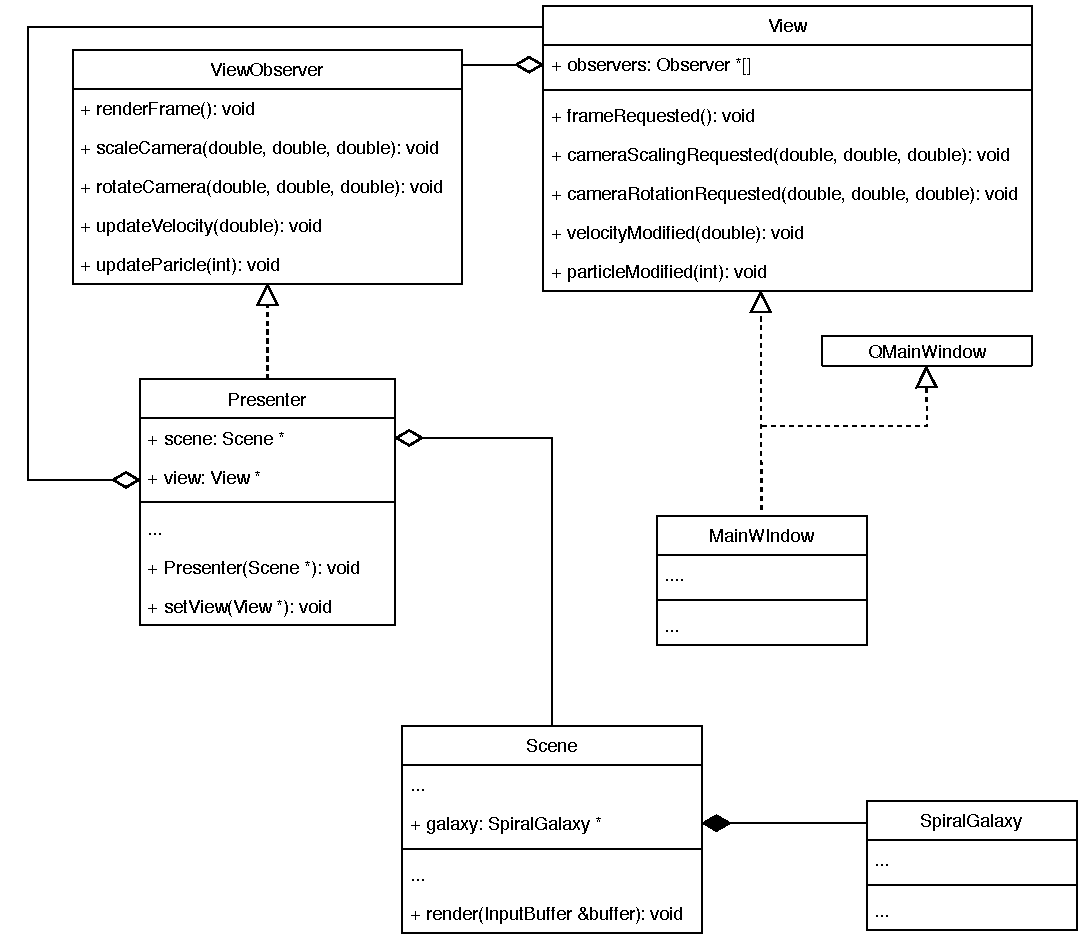
\includegraphics[scale=0.8]{pdf/mvp_uml.pdf}
    \caption{Диаграмма Сущность-Связь приложения}
    \label{img:mvp_uml}
\end{figure}

\section{Описание пользовательского интерфейса}
На рисунке \ref{img:gui01} изображён снимок экрана с интерфейсом готового приложения, который позволяет пользователю изменить скорость вращения спиральных рукавов или количество частиц в системе.
\begin{figure}[H]
    \centering
    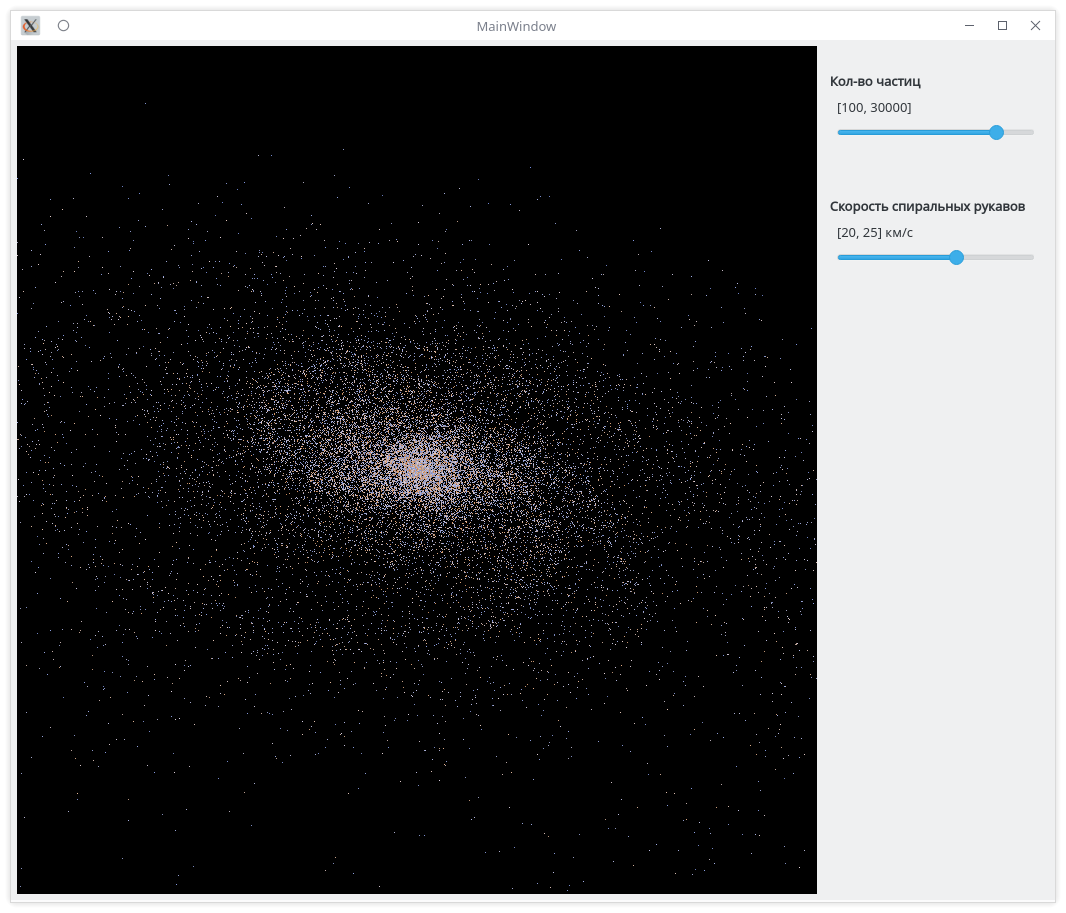
\includegraphics[scale=0.5]{image/gui01.png}
    \caption{Интерфейс разработанного приложения}
    \label{img:gui01}
\end{figure}

Для приближения предназначена клавиша ``='', для отдаления - ``-''. Вращения вокруг оси Z осуществляется при помощи клавиш ``Q'' и ``E'', вокруг оси Y - ``W'' и ``S'', вокруг оси X - ``A'' и ``D''.

\section{Тестирование}
Было проведено функциональное тестирование белого ящика, в ходе которого программа отработала правильно. Также проведено тестирование пользовательского интерфейса, все элементы интерфейса реагируют корректно.

\section{Вывод}
На языке C++ были реализованы алгоритмы моделирования и визуализации спиральной галактики. Программа полностью прошла функциональное тестирование и тестирование интерфейса.

